\section{Man against machine}
\label{sect:mam_study}
\subsection{Introduction}
Selecting appropriate groups to perform is a complex task. There are many trade-offs to be made between the various competing preferences and constraints. When the schedule is heavily loaded, i.e. there are potentially more observations to perform than could be accomodated even under ideal conditions, the job of the scheduler becomes both simpler and more difficult. It is relatively \emph{easy} to find a solution which satisfies the constraints, however finding an optimal solution is rendered more \emph{difficult} due to the number of potential solutions to compare. 

A major problem is to determine just what those trade-offs are. We would like to be able to answer questions like:- \emph{how much more important is a high priority, non-urgent group relative to a medium priority, urgent group ?}. It is because it is difficult to quantify these relative weights that we turn to the human scheduler. A human makes these sort of trade-offs on a daily basis - often with little knowledge they are doing it. If we set up a human to perform the task we might be able to deduce from what they have done and the choices they have made some of the rules they are using (often without realizing) and the relative weighting they employ. Additionally, it was thought this might yield a useful baseline for the automated schedulers.

Two sets of trials are performed. Firstly the human scheduler (referred to as HS) is presented with a snapshot of the ODB content for the trial night in a tabular format  from which to generate a schedule. Secondly a set of simulations are run in which the relative scoring weights are changed to try and reproduce the results of HS and ideally to beat them.

\subsection{Characterization of problem}
On the night of the test (13-14 November 2007) there are some 13.33 hours of night (including twilight time) with additonal details in Table.~\ref{tab:mam_nights}.
The supplied ODB snapshot consists of 131 groups and a total of 2880.32 minutes (48 hours) of available observing time in the night, an oversubscription factor of 3.6

\begin{table}[htbp]
\begin{center}
\begin{tabular}{lll}
\toprule
\multicolumn{3}{c}{Case study night characteristics} \\
\midrule
Item       &  Time               & Lunar elevation \\
\midrule
Sunset     & 2007-11-13 18:15 UT & 23.4$^{\circ}$\\
StartNight & 2007-11-13 19:40 UT & 11.2$^{\circ}$\\
Moonset    & 2007-11-13 20:50 UT & 0.0$^{\circ}$\\
EndNight   & 2007-11-14 06:05 UT & -66.0$^{\circ}$\\
Sunrise    & 2007-11-14 07:35 UT & -47.3$^{\circ}$\\
\midrule
Item                         & Duration (hours) \\
\midrule
Length of dark night         & 10.42\\
Length of night inc twilight & 13.33\\
\bottomrule
\end{tabular}
\caption[Characteristics of test night for HS1 experiment]{Characteristics of the test night for HS1 experiment.}
\label{tab:mam_nights}
\end{center}
\end{table}


The groups within the snapshot are distributed throughout the range of priority as shown in Table~\ref{tab:priority_distrib}. Excluding the background groups, which should only run as a last resort and do not contribute to the science program, there are a total of 34.8 hours giving a more realistic oversubscription factor of 2.6.

% GROUP PRIORITY DISTRIBUTION
\begin{table}
\begin{center}
\begin{tabular}{llp{6cm}}
\toprule
\multicolumn{3}{c}{ODB snapshot characteristics} \\
\midrule
Priority & $N_G$ & $\sum{X_g}$ (hours)\\
\midrule
0 & 1 & 2.8\\
1 & 55 & 1190.1\\
2 & 26 & 462.3\\
3 & 12 & 169.5\\
5 & 2  & 39.4\\
BG & 23 & 790.3\\
STD & 12 & 226.8\\
\midrule
Total & 131 & 2880.3\\
\bottomrule
\end{tabular}
\caption[Distribution of number of groups between priority levels for HS1 experiment]{Distribution of number of groups $N_G$ and total executable time $\sum{X_g}$ among the available priority levels. Priority 1 and 2 make up the bulk of the science groups with relatively few high priority groups. Background (BG) and standard (STD) groups are not part of the science program.}
\label{tab:priority_distrib}
\end{center}
\end{table}

Figures~\ref{fig:mam_h1_contention} and \ref{fig:mam_h1_dmd} show respectively the contention and demand plots for the night. The predicted contention $C_c$ is very high at around 90 for much of the night. A simulation run with a \emph{typical} scheduler, shown on the same plot shows the actual contention dropping from around 80 to 40 over the course of the night. The total demand $C_d$ remains fairly constant at a level of around 4 to 5 for the night while the urgency-weighted demand $C_{ud}$ rises from 1 to nearly 2 over the course of the night. This latter indicates that selection of just the urgent groups would likely fill most of the available observing time.

\begin{figure}[htbp]
\begin{center}
    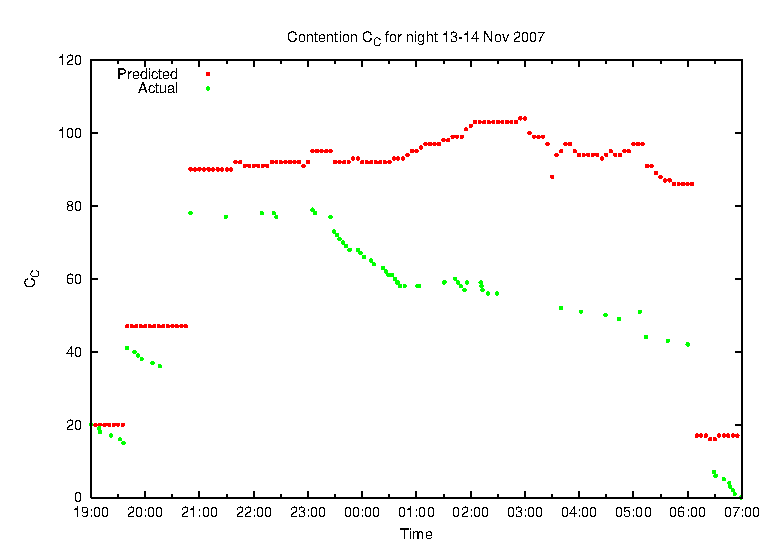
\includegraphics[scale=1.0, angle=0]{figures/mam/cont.eps}
\end{center}
\caption[Contention for night 13-14 November 2007.]
{Contention for night 13-14 November 2007 for H1 test. The two plots show the expected contention based on ODB content calculated in advance and the actual contention derived during a typial scheduling run on the night.}
\label{fig:mam_h1_contention}
\end{figure}

\begin{figure}[htbp]
\begin{center}
    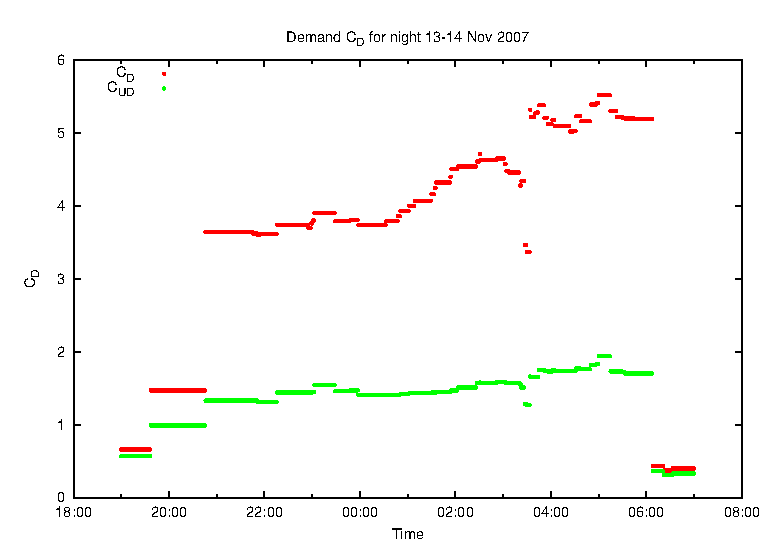
\includegraphics[scale=1.0, angle=0]{figures/mam/dmd.eps}
\end{center}
\caption[Demand for night 13-14 November 2007.]
{Demand for night 13-14 November 2007 for H1 test. The two plots show the overall and urgency-weighted demand.}
\label{fig:mam_h1_dmd}
\end{figure}


\subsection{Human scheduling trial (HS1)}
A human subject (expert scheduler) is provided with information concerning which groups are potentially feasible on the test night. An example section of the data provided is shown in Table.~\ref{tab:example_gen}. The information, described in Table.~\ref{tab:hsgexample} contains details of the target, timing and observing constraints along with a simple pre-calculated feasibility plot for the night for each group. Some metrics are also available. The urgency metric indicates on how many remaining nights the group might be observed. The execution-time metric indicates the expected execution time of the group. 

In light of the difficulty for a human to generate the schedule by collating the considerable amount of information available a number of the normal constraints were relaxed. e.g. it is not easy for a human to keep precise track of the accumulating time to the second so execution times are given to the nearest minute. The accuracy of the availability plot is also shown only to around 5-10 minutes so when testing the feasibility (in terms of target elevation) a few degrees of leeway are given. In order to uncomplicate the scenario the assumption is also made that seeing is good for the whole night. 

The HS uses the information to devise a schedule for the night by recording the start time and ID of each group to execute in order. Due to the time taken to perform one of these HS trials - several hours, only a single trial (HS1) was performed.


\begin{table}
\begin{center}
\begin{tabular}{|l|l|l|p{6cm}|}
\hline
{\bf Column} & {\bf Title}  & {\bf Example} & {\bf Description}\\
\hline
1  & Numeric ID     & G\_476          & Used by HS to mark up the schedule.\\
2  & Target RA      & 0:42:49.64      & RA in (hh:mm:ss) format.\\
3  & Target Dec     & 41:15:26.50     & Declination in (dd:mm:ss) format.\\
4  & Group Name     & ANGM31          & The actual name of the group.\\
5  & Timing         & MONITR 2.5H [2] & Class of timing constraint.\\
6  & Moon OC        &                 & Observability with moon risen.\\
7  & Seeing OC      & POOR            & Minimum seeing category.\\
8  & Solar Elev OC  &                 & Observability in twilight.\\
9  & Priority       & 2               & TAG assigned priority.\\
10 & Execution Time & 33.4M           & Expected time to run.\\
11 & Urgency        & CRIT              & Remaining observable nights.\\
12 & Availability   & \_\_9**********\_ & Display of observability. \\

\hline

\end{tabular}
\caption{Description of the columns in the table provided to the human scheduler.}
\label{tab:hsgexample}
\end{center}
\end{table}

\clearpage

\begin{landscape}

\begin{table}[h!]
  \begin{center}
  \end{center}
  \caption{Sample section of table available to HS.}
  \label{tab:example_gen}
\end{table}

\scriptsize
\begin{verbatim}

G_276     3:24:44.055  50:11:21.63  com17Pmon-071030    MONITR 48H [36]                     POOR ASTR  P= 1   XT= 2.25M    RN= CRIT 3***********9_
G_355     3:13:24.16   18:49:38.40  FS109               MONITR 3H [1]                       POOR ASTR  P= STD XT= 4.6M     RN= CRIT _5*********7__
G_369     3:24:7.995   50:9:33.39   17P-mosaic          FLEXBL                              AVER ASTR  P= 3   XT= 13.73M   RN= 21   3***********9_
G_370     3:24:7.995   50:9:33.39   17P-monitor         MONITR 3H [2]                       AVER NAUT  P= 2   XT= 3.63M    RN= CRIT 3***********9_
G_025     4:9:17.00    30:46:33.00  932a000t000         FLEXBL                         DARK POOR       P= 1   XT= 3.27M    RN= 17   __9**********_
G_028     4:30:14.00   35:16:10.00  927e000t000         FLEXBL                         DARK POOR       P= 1   XT= 3.27M    RN= 17   __7**********5
G_093     5:34:32.00   22:0:52.00   927h000t000         FLEXBL                         DARK POOR       P= 1   XT= 3.27M    RN= 16   ___2**********
G_382     5:5:30.60    52:49:54.00  zero_G191B2         MONITR 5H [3]                       POOR       P= STD XT= 3.53M    RN= CRIT __7***********
G_048     6:54:18.125  24:40:7.32   725d000t000         FLEXBL                              POOR ASTR  P= 1   XT= 1.27M    RN= 19   _____*********
G_408     6:54:18.12   24:40:7.38   927c000t000         FLEXBL                              POOR ASTR  P= 2   XT= 1.27M    RN= 19   _____*********
G_002     7:24:18.00  -0:32:17.00   Photom_G1_RU149     INTVAL 3H                           POOR ASTR  P= STD XT= 9.87M    RN= ICRT ______6*******
G_126     7:8:0.77     22:31:14.50  FocusShort_07       MONITR 168H [167]                   POOR ASTR  P= BGR XT= 7M       RN= 7    _____7********
G_284     7:23:44.00   20:25:6.00   mho_monitor         INTVAL 22.5H                        POOR       P= 1   XT= 71.1M    RN= ICRT _____4********
G_352     7:24:14.40  -0:33:4.10    FS14                MONITR 3H [1]                       POOR ASTR  P= STD XT= 5.43M    RN= CRIT ______6*******
G_371     7:36:51.00   65:36:7.00   lens_2403           MONITR 48H [36]                     POOR       P= 2   XT= 15.07M   RN= CRIT ____9*********
G_259     8:6:11.10   -27:31:42.00  ESO494-G26          FLEXBL                         DARK POOR       P= 1   XT= 22.17M   RN= 11   ________4*****
G_358     8:6:23.70    20:6:31.90   J0806               INTVAL 96H                          POOR       P= 3   XT= 27.33M   RN= 17   ______6*******
G_472     8:54:48.90   20:6:30.64   0851                MONITR 168H [167]              DARK AVER       P= 1   XT= 7.8M     RN= 3    _______8******
G_237     9:17:21.90   41:54:38.00  UGC4904             FLEXBL                         DARK POOR       P= 1   XT= 22.17M   RN= 13   ______1*******
G_260     9:32:6.20    8:26:31.00   NGC 2906            FLEXBL                         DARK POOR       P= 1   XT= 23.83M   RN= 12   ________8*****
G_263     9:45:48.30  -14:22:6.00   NGC2993             FLEXBL                         DARK POOR       P= 1   XT= 22.17M   RN= 10   _________7****
G_266     9:54:28.60  -25:42:12.00  NGC3054             FLEXBL                         DARK POOR       P= 1   XT= 23.83M   RN= 9    __________8***
G_280     9:50:31.97  -2:49:47.20   group07b01c         FLEXBL                         DARK AVER       P= 1   XT= 28.8M    RN= 11   ________1*****
G_281     9:47:51.21  -2:24:18.80   group07b01b         FLEXBL                         DARK AVER       P= 1   XT= 28.8M    RN= 11   ________2*****
G_373     9:55:33.20   69:3:55.00   lens_M81            MONITR 48H [36]                     POOR       P= 2   XT= 15.07M   RN= CRIT ______8*******
G_004     10:50:5.70  -0:1:12.00    Photom_G1_1047+003  INTVAL 3H                           POOR ASTR  P= STD XT= 9.63M    RN= ICRT _________2****
G_265     10:52:11.40  32:57:2.00   NGC 3430            FLEXBL                         DARK POOR       P= 1   XT= 23.83M   RN= 11   ________3*****
G_282     10:11:42.74 -2:58:16.90   group07b01d         FLEXBL                         DARK AVER       P= 1   XT= 28.8M    RN= 10   _________8****
G_407     10:39:57.45  10:4:0.47    926j000t000         FLEXBL                              POOR ASTR  P= 2   XT= 1.31M    RN= 19   _________8****
G_213     11:32:2.40   36:41:53.00  UGC6517             FLEXBL                         DARK POOR       P= 1   XT= 22.17M   RN= 10   _________7****
G_244     11:25:2.50  -9:47:43.00   NGC3672             FLEXBL                         DARK POOR       P= 1   XT= 22.17M   RN= 9    __________2***
G_353     11:37:5.15   29:47:58.40  FS21                MONITR 3H [1]                       POOR ASTR  P= STD XT= 5.43M    RN= CRIT _________4****
G_204     12:52:34.70 -9:46:36.00   MCG-01-33-34        FLEXBL                         DARK POOR       P= 3   XT= 23.83M   RN= 4    ____________8*
G_210     12:5:34.20   50:32:21.00  NGC4088             FLEXBL                         DARK POOR       P= 1   XT= 22.17M   RN= 10   _________6****
G_218     12:2:12.20   62:8:14.00   NGC4041             FLEXBL                         DARK POOR       P= 1   XT= 22.17M   RN= 11   ________2*****
G_245     12:48:13.60 -3:19:58.00   NGC4691             FLEXBL                         DARK POOR       P= 1   XT= 23.83M   RN= 9    ___________1**
G_439     13:6:56.00   29:34:48.00  z2_1_H13            MONITR 672H [599.98]           DARK POOR       P= BGR XT= 49.73M   RN= 5    ___________9**
G_440     13:6:56.00   29:34:48.00  z1_1_H13            MONITR 672H [599.98]           DARK POOR       P= BGR XT= 49.73M   RN= 5    ___________9**
G_360     14:6:24.82   61:26:40.90  J1406               INTVAL 72H                          POOR       P= 3   XT= 27.33M   RN= 21   2_________1***
\end{verbatim}
\end{landscape}
\normalsize

%G_481     14:17:59.60  25:6:53.00   5548_opt            MONITR 168H [120]                   POOR ASTR  P= 2   XT= 3.13M    RN= 3    ____________6*
%G_427     16:35:15.49  38:8:4.50    darkbias_16h        MONITR 24H [22.97]                  POOR ASTR  P= 2   XT= 4.34M    RN= CRIT *7____________
%G_275     17:57:48.00  4:42:48.50   TST-BarnStar-071105 FLEXBL                              POOR       P= 0   XT= 2.8M     RN= 10   **____________
%G_365     19:0:34.78   22:34:54.10  Focus19_zr          INTVAL 12H                          AVER CIVT  P= BGR XT= 9.9M     RN= ICRT ***7__________
%G_366     19:0:34.78   22:34:54.10  Focus19_rr          INTVAL 168H                         AVER CIVT  P= BGR XT= 9.8M     RN= 21   ***7__________
%G_367     19:0:34.78   22:34:54.10  Focus19_Br          INTVAL 12H                          AVER CIVT  P= BGR XT= 11.18M   RN= ICRT ***7__________



\subsection{Results of HS1 trial}
The analysis proceeds as follows:- For each scheduled (group ID, start-time) pair, the feasibility is worked out for that time. This consists of testing the target elevation against dome limit (20 degs) and the group constraints on moon and sun elevation against actual elevations. If the schedule is feasible, the various quality metrics are then computed.

The HS1 experiment yielded a run of 147 group executions. There were a total of 9 overruns of respectively (1,1,1,1,3,4,5,10,10) minutes, there were considered sufficiently minor to be ignored. A preliminary look at the scoring profile shows the value of $elevation/transit\_height$ to be generally high - suggesting the human scheduler has tried to observe targets as they cross the zenith. There are 2 instances of targets observed below the horizon - one of these at -60 degrees elevation ! - possibly a misreading of a declination ?. This value was removed from the final results to avoid skewing.

\subsection{Simulation trials}
Several simulation trials were performed using a basic despatch scheduler (BDS) and several configurations of a look-ahead scheduler (QLAS). The BDS simulations were performed using different weighted scoring functions. The QLAS simulations were performed using horizons of 1, 2, 4 and 8 hours and using search parameters of 100, 250 and 2500 trials. Each simulation was run 100 times to obtain statistical values for the various Q metrics.

A first set of trials were run using the scoring function $w_{el}f_{el}+(1-w_{el})f_{pr}$ with $w_{el}$ ranging from 0.0 to 1.0. With $w_{el}=0$ the scoring is purely based on priority. At the other extreme ($w_{el}=1$) the scoring is purely based on target elevation. Plots of the quality metrics $Q_{el}$ and $Q_{pr}$ against $w_{el}$ are shown in Figures.~\ref{fig:bdsqel} and \ref{fig:bdsqpr}. The results of HS1 and BDS simulations with a random selection model are plotted for comparison. From Fig.~\ref{fig:bdsqel} it is clear that random selection is always a poorer option. The HS wins over BDS when $w_{el}$ is small (priority-dominated selection) and only after $w_{el}>0.9$ is BDS better - this suggests that the HS is quite elevation-dominated. Inspection of Fig.~\ref{fig:bdsqpr} shows again that random selection is a poor choice. However we also see that HS beats BDS only when $w_{el}$ exceeds 0.7, suggesting that HS has a lower degree of priority bias. From this we may conclude that HS is using a scoring criterion with a large value of $w_{el}$ and a somewhat lower value of $w_{pr}$ though it is not feasible to determine exactly what these are.

A further series of simulations were performed using BDS with fixed values of $w_{el}$ and $w_{pr}$ to guage the variation in results. The results for these are shown in Table.~\ref{tab:hsbdscomp}. The column labelled {\bf h1} represents HS1. The various columns labelled $\mathbf{B_a}$ represent the use of BDS with scoring based solely on metric $f_a$. The columns $\mathbf{B_{x,y}}$ represent BDS scored using a combination of $f_{pr}$ and $f_{el}$ in the proportion $(xf_{el}+yf_{pr})/10$. 

The scheduler $B_{el}$ achieves the best results for $Q_{el}$ as might be expected. Interestingly it performs slightly less well than HS on $Q_{rn}$ and $Q_{td}$, and indeed HS performs better on this metric than any BDS implementations including $B_{rn}$. This suggests there may be an element of \emph{urgency-weighting} in HS. $B_{pr}$ performs best on $Q_{pr}$, however, surprisingly slightly less well than HS overall on this metric. HS holds its own against all the BDS implementations on the other quality metrics with the exception of $Q_{td}$ where $B_{td}$ performs twice as well as anything else. The overall modified conclusion then is that HS uses a selection criterion along the lines of $w_{el}f_{el}+w_{pr}f_{pr}+w_{rn}f_{rn}$ in which $w_{el}$ dominates, $w_{pr}$ is next highest and $w_{rn}$ is somewhat smaller. Inspection of the table columns shows the scheduler $B_{8,2}$ comes fairly close to matching the HS column giving $w_{el}=0.8$ and $w_{pr}=0.2$.



\begin{figure}[htbp]
  \begin{center}
    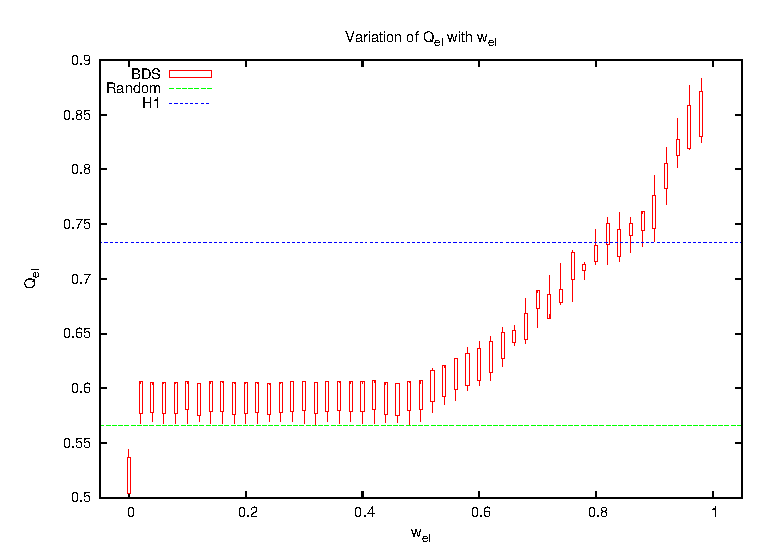
\includegraphics[scale=1.0, angle=0]{figures/cmp_el.eps}
  \end{center}
  \caption[Variation of $Q_{el}$ with $w_{el}$ for BDS simulations.]
  {Variation of $Q_{el}$ with $w_{el}$ for BDS simulations with scoring funtion $w_{el}f_{el}+(1-w_{el})f_{pr}$. Plots labelled \emph{H1} and \emph{Random} represent the results for HS1 and for BDS with a random selection model.}
  \label{fig:bdsqel}
\end{figure}
  
\begin{figure}[htbp]
  \begin{center}
    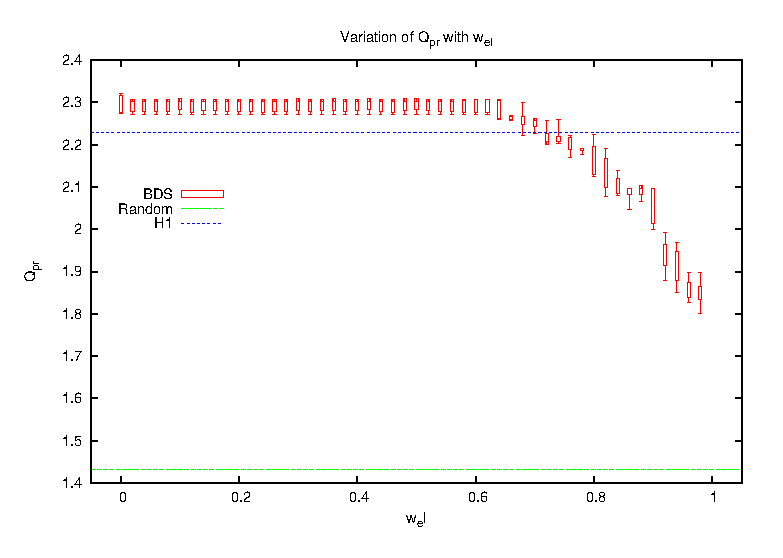
\includegraphics[scale=1.0, angle=0]{figures/cmp_pr.eps}
  \end{center}
  \caption[Variation of $Q_{pr}$ with $w_{el}$ for BDS simulations.]
  {Variation of $Q_{pr}$ with $w_{el}$ for BDS simulations with scoring funtion $w_{el}f_{el}+(1-w_{el})f_{pr}$. Plots labelled \emph{H1} and \emph{Random} represent the results for HS1 and for BDS with a random selection model}
  \label{fig:bdsqpr}
\end{figure}
  
\clearpage

\begin{table}[hbtp]

  \subtable [Results of BDS simulations and Human scheduler] {
    \label{tab:hsbdscomp}
    \begin{tabular}{|l|rrrrrrrrr|}
     \hline
     {\bf metric} & {\bf $h_1$} & {\bf $B_{el}$} &  {\bf $B_{pr}$} & {\bf $B_{rn}$} & {\bf $B_{td}$} & {\bf $B_{2,8}$} & {\bf $B_{5,5}$} & {\bf $B_{8,2}$} & {\bf $B_{rnd}$}\\
     \hline
     {\bf $Q_{el}$} & 0.77 & 0.88 & 0.52 & 0.36 & 0.4  & 0.59 & 0.58 & 0.72 & 0.56 \\
     {\bf $Q_{pr}$} & 2.34 & 1.87 & 2.29 & 1.73 & 1.54 & 2.3  & 2.3  & 2.16 & 1.43 \\
     {\bf $Q_{sm}$} & 0.28 & 0.3  & 0.26 & 0.28 & 0.32 & 0.25 & 0.25 & 0.25 & 0.33 \\
     {\bf $Q_{lm}$} & 0.71 & 0.8  & 0.68 & 0.82 & 0.92 & 0.64 & 0.63 & 0.7  & 0.86 \\
     {\bf $Q_{rn}$} & 0.67 & 0.48 & 0.4  & 0.58 & 0.4  & 0.47 & 0.47 & 0.45 & 0.35 \\
     {\bf $Q_{td}$} & 0.07 & 0.06 & 0.05 & 0.1  & 0.12 & 0.06 & 0.06 & 0.05 & 0.08 \\
     {\bf $Q_{xt}$} & 0.99 & 0.99 & 0.96 & 0.99 & 1.0  & 0.96 & 0.97 & 0.96 & 1.0  \\
     \hline
   \end{tabular}
  }

%\subsection{LAS simulation results}
%extra features - bg selection thresh - other wise stay idle, overun thresh frac of group in horizon

  \subtable [Results of LAS simulations and Human scheduler (n=100)] {
    \label{tab:lascomp1}
    \begin{tabular}{|l|r|rrrr|}
      \hline
     {\bf metric} & {\bf $h_1$} & {\bf 1} & {\bf 2} &  {\bf 4} & {\bf 8} \\
     {\bf $Q_{el}$} & 0.77 & 0.574 &0.569 &0.579 &0.571\\
     {\bf $Q_{pr}$} & 2.34 & 1.848 &1.801 &1.811 &1.812\\
     {\bf $Q_{sm}$} & 0.71 & 0.815 &0.820 &0.847 &0.839\\
     {\bf $Q_{lm}$} & 0.28 & 0.317 &0.321 &0.325 &0.327\\
     {\bf $Q_{rn}$} & 0.67 & 0.362 &0.344 &0.347 &0.358\\
     {\bf $Q_{xt}$} & 0.99 & 1.000 &0.998 &1.012 &1.007\\
     \hline
    \end{tabular}
  }

  \subtable [Results of LAS simulations and Human scheduler (n=500)] {
    \label{tab:lascomp2}
    \begin{tabular}{|l|r|rrrr|}
      \hline
      {\bf metric} & {\bf $h_1$} & {\bf 1} & {\bf 2} &  {\bf 4} & {\bf 8} \\
      {\bf $Q_{el}$} &  0.77 & 0.569 &0.576 &0.584 &0.584\\
      {\bf $Q_{pr}$} & 2.34  &1.863 &1.818 &1.790 &1.807\\
      {\bf $Q_{sm}$} &  0.71 &0.816 &0.831 &0.838 &0.843\\
      {\bf $Q_{lm}$} & 0.28  &0.311 &0.326 &0.329 &0.330\\
      {\bf $Q_{rn}$} & 0.67  & 0.345 &0.357 &0.356 &0.344\\
      {\bf $Q_{xt}$} & 0.99  &0.994 &1.010 &1.016 &1.011\\
      \hline
    \end{tabular}
  }

  \subtable [Results of LAS simulations and Human scheduler (n=2500)] {
    \label{tab:lascomp3}
    \begin{tabular}{|l|r|rrrr|}
      \hline
      {\bf metric} & {\bf $h_1$} & {\bf 1} & {\bf 2} &  {\bf 4} & {\bf 8} \\
      {\bf $Q_{el}$} &  0.77 & 0.573 &0.577 & 0.58 & 0.582\\
      {\bf $Q_{pr}$} & 2.34  &1.855 &1.826 & -&-\\
      {\bf $Q_{sm}$} &  0.71 &0.837 &0.838 & -&-\\
      {\bf $Q_{lm}$} & 0.28  &0.324 &0.327 & -&-\\
      {\bf $Q_{rn}$} & 0.67  &0.340 &0.342 & -&-\\
      {\bf $Q_{xt}$} & 0.99  &1.013 &1.011 & -&-\\
      \hline
    \end{tabular}
  }
\end{table}

